\documentclass[pointlessnumbers, abstracton, headsepline, a4paper]{scrartcl}

\usepackage[T1]{fontenc}
\usepackage[utf8]{inputenc}
\usepackage{graphicx}
\usepackage{microtype}
\usepackage{textcomp}
\usepackage{ellipsis, fixltx2e, mparhack, booktabs, longtable}
\usepackage[automark]{scrpage2}
\usepackage{multicol}
\usepackage{microtype}
\usepackage{listings}
\usepackage[a4paper]{geometry}
\usepackage[polish]{babel}
\usepackage{subfigure}
\usepackage{tikz}
\usetikzlibrary{arrows,positioning}

\usepackage{courier}
\lstset{
         basicstyle=\footnotesize\ttfamily, % Standardschrift
         %numbers=left,               % Ort der Zeilennummern
         numberstyle=\tiny,          % Stil der Zeilennummern
         %stepnumber=2,               % Abstand zwischen den Zeilennummern
         numbersep=5pt,              % Abstand der Nummern zum Text
         tabsize=2,                  % Groesse von Tabs
         extendedchars=true,         %
         breaklines=true,            % Zeilen werden Umgebrochen
         keywordstyle=\color{red},
         stringstyle=\color{white}\ttfamily, % Farbe der String
         showspaces=false,           % Leerzeichen anzeigen ?
         showtabs=false,             % Tabs anzeigen ?
         showstringspaces=false      % Leerzeichen in Strings anzeigen ?        
}

% part of the hyperref bundle
\usepackage{ifpdf}

\geometry{verbose,tmargin=3.5cm,bmargin=3.5cm}
\setlength{\parskip}{\medskipamount}
\setlength{\parindent}{0pt}

\clearscrheadfoot
\ohead{\\\headmark}
\ihead{
\includegraphics[scale=0.2]{img/zut2.jpg}}
\ofoot[\pagemark]{\pagemark}

% if pdflatex is used
\ifpdf

%set fonts for nicer pdf view
\IfFileExists{lmodern.sty}{\usepackage{lmodern}}
  {\usepackage[scaled=0.92]{helvet}
    \usepackage{mathptmx}
    \usepackage{courier} }
\fi

% the pages of the TOC are numbered roman
% and a pdf-bookmark for the TOC is added
\pagenumbering{arabic}
\let\myTOC\tableofcontents
\renewcommand\tableofcontents{\myTOC\clearpage\pagenumbering{arabic}}

\begin{document}
\begin{titlepage}

\begin{center}

\includegraphics[scale=0.5]{logos/zut.jpg}
\par
\end{center}

\begin{center}
\textsf{\textbf{\LARGE Wydział Informatyki}}
\end{center}{\LARGE}

\vspace{1.5cm}

\begin{center}
\textsf{\Large Metody sztucznej inteligencji}
\end{center}

\begin{center}
\textsf{\textbf{\Large Laboratorium 02 IUz-22 Urbaniak}}
\end{center}

\begin{center}
\textsf{\large Sprawozdanie}
\end{center}

\vspace{3.5cm}

\begin{center}
\begin{tabular}{ll}
Autor: & Sergiusz Urbaniak\tabularnewline
Grupa: & IUz-22\tabularnewline
Data: & \today\tabularnewline
\end{tabular}
\end{center}

\end{titlepage}

\tableofcontents

\section{Wprowadzenie}
Następujące zadania nie zostały rozwiązane za pomocą oprogramowania Matlab lecz dzięki alternatywnych i wolnodostępnych rozwiązań. Jest to spowodowane faktem że autor niestety nie posiada stałego dostępu do internetu i jest skazany do odrabiania sprawozdań "w drodze" (w pociągach). Poza tym jest zwolennikiem "Open Source".

Istnieje ciekawy projekt o nazwie FANN (Fast Artificial Neural Network Library)\footnote{http://leenissen.dk/fann}. Biblioteka ta udostępnia algorytmy związane z sieciami neuronowymi pod różnymi językami. Dla następującego sprawozdania został wybrany język Python. Jest to język przede wszystkim obiektowy (w odróżnieniu do języka w Matlabie/Octavie) i posiada znakomite biblioteki naukowe (scipy, numpy, matplotlib).

\section{Bramka logiczna XOR}

Bramka XOR posiada tablice prawdy pokazaną w tablicy \ref{tab:xor}.

\begin{table}[h]
\centering
\begin{tabular}[t]{c|c}
Wejście & Wyjście \\
\hline
0 0 & 0 \\
0 1 & 1 \\
1 0 & 1 \\
1 1 & 0 \\
\end{tabular}
\caption{\label{tab:xor}Tablica prawdy bramki XOR}
\end{table}

Zamodelowac można ją za pomocą dwóch neuronów w warstwie ukrytej. Sieć neuronowa jest pokazana w rysunku \ref{fig:xor}.

\begin{figure}[!h]
\centering
\def\layersep{2.5cm}

% Define two helper counters
\begin{tikzpicture}[shorten >=1pt,->,draw=black!50, node distance=\layersep]
    \tikzstyle{every pin edge}=[<-,shorten <=1pt]
    \tikzstyle{neuron}=[circle,fill=black!25,minimum size=17pt,inner sep=0pt]
    \tikzstyle{input neuron}=[neuron, fill=green!50];
    \tikzstyle{output neuron}=[neuron, fill=red!50];
    \tikzstyle{hidden neuron}=[neuron, fill=blue!50];
    \tikzstyle{annot} = [text width=4em, text centered]

    % Draw the input layer nodes
    \foreach \name / \y in {1,...,2}
    % This is the same as writing \foreach \name / \y in {1/1,2/2,3/3,4/4}
        \node[input neuron, pin=left:Wejście \#\y] (I-\name) at (0,-\y) {};

    % Draw the hidden layer nodes
    \foreach \name / \y in {1,...,2}
        \path
            node[hidden neuron] (H-\name) at (\layersep,-\y cm) {};

    % Draw the output layer node
    \node[output neuron,pin={[pin edge={->}]right:Wyjście}] (O) at (\layersep*2, -1.5 cm) {};

    % Connect every node in the input layer with every node in the
    % hidden layer.
    \foreach \source in {1,...,2}
        \foreach \dest in {1,...,2}
            \path (I-\source) edge (H-\dest);

    % Connect every node in the hidden layer with the output layer
    \foreach \source in {1,...,2}
        \path (H-\source) edge (O);

    % Annotate the layers
    \node[annot,above of=H-1, node distance=1cm] (hl) {Ukryta warstwa};
    \node[annot,left of=hl] {Wejściowa warstwa};
    \node[annot,right of=hl] {Wyjściowa warstwa};
\end{tikzpicture}

\caption{\label{fig:xor}Siec neuronowa wielowarstwowa}
\end{figure}

Nie uczona sieć jest widoczna w rysunku \ref{fig:xor_unlearned}. W diagramie widać na czerwonych punktach właściwe dane wyjściowe. Na zielonych punktach widoczna jest wyjście z sieci. Można zauważyć że istnieje błąd widoczny w dolnym diagramie.

\begin{figure}[!h]
\centering
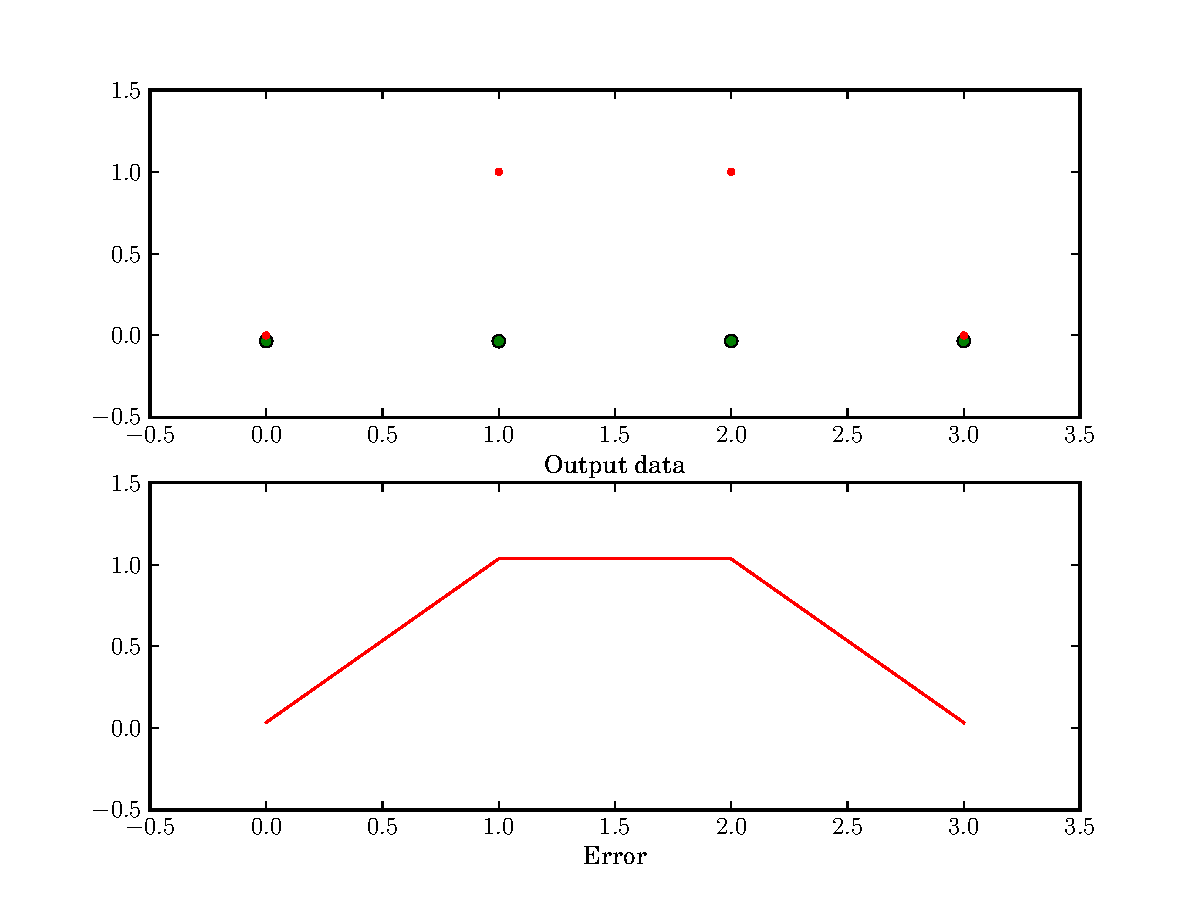
\includegraphics[scale=0.8]{src/xor/xor_untrained.pdf}\caption{\label{fig:xor_unlearned}Wyniki przed uczeniu}
\end{figure}

Wynik po uczeniu widać na rysunku \ref{fig:xor_learned}. Widać że siec z tylko dwoma neuronami była w stanie nauczyć się bramki XOR. Wyjście sieci (zielone punkty) zbliżyły się do właściwych wartości i błąd wynosi 0.

\begin{figure}[!h]
\centering
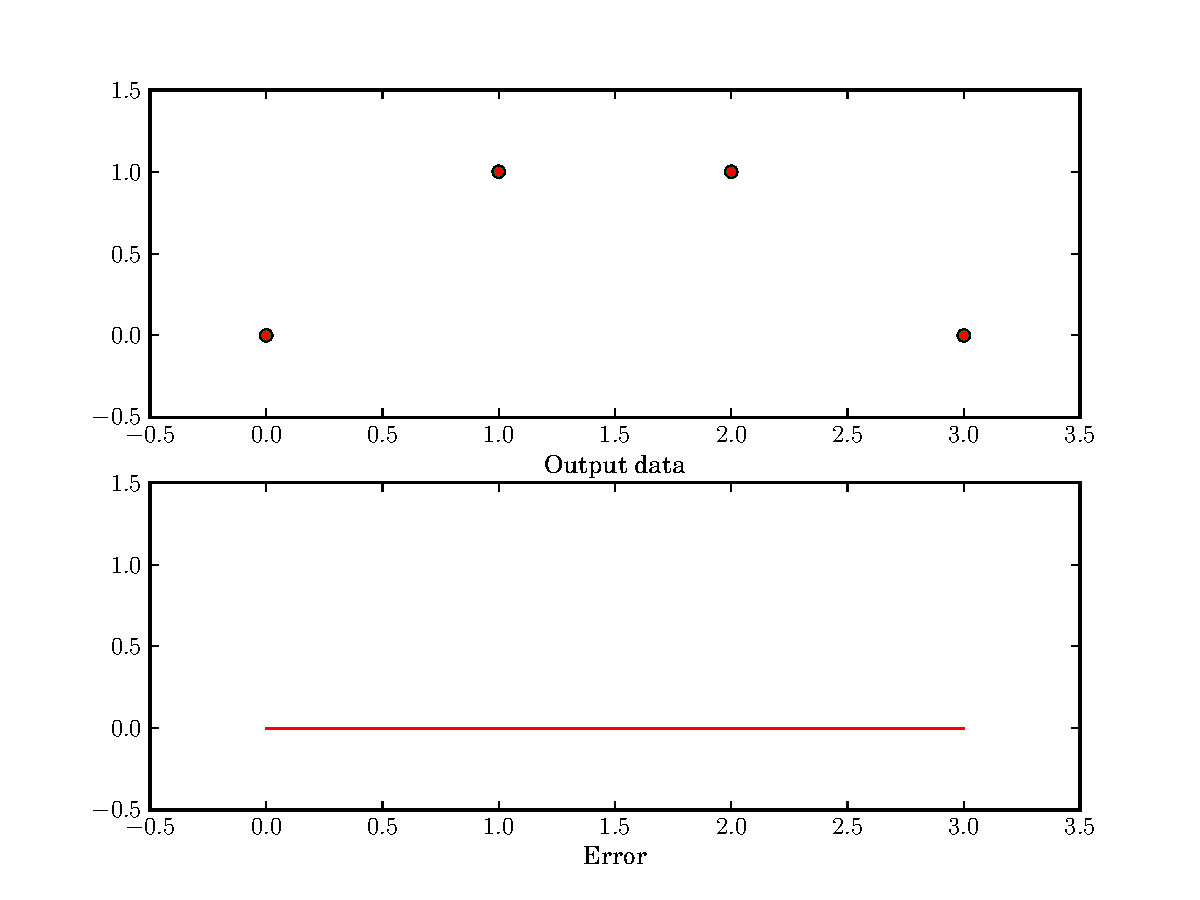
\includegraphics[scale=0.8]{src/xor/xor_trained.pdf}\caption{\label{fig:xor_learned}Wyniki po uczeniu}
\end{figure}

Kod uczenia jak i wykresów jest widoczny w listingu \ref{lst:xor.py}.

\clearpage
\begin{center}
\lstset{captionpos=b,caption=Kod uczenia bramki XOR,label=lst:xor.py}
\lstinputlisting{src/xor/xor.py}
\end{center}

\clearpage
\section{Uczenie plików}
Uczenie podanymi plikami okazało się już trudniejszym zadaniem. Okazało się że siec zbudowana z FANN zbyt nie dokładnie się uczy danych. Wybrano jednak te pliki gdzie uzyskano najmniejsze błędy. Zostały wybrane następujące zestawy:

\begin{itemize}
\item parity\_i.txt, parity\_o.txt
\item sincos\_i, sincos\_o.txt
\item glass.txt
\end{itemize}

Następujące rozdziały są organizowane w trzy części:
\begin{enumerate}
\item Opis optymalnych danych dla danego pliku
\item Tabela badań z różnymi funkcjami aktywacji. Skonfigurowano bibliotekę FANN w taki sposób aby przestała uczyć siec jak wystąpi jeden z następujących warunków:
\begin{itemize}
\item Aktualna iteracja (epoka) wynosi nie więcej niż 1000
\item Błąd jest poniżej 0.0001
\end{itemize}
\item Wykresy badan:
\begin{itemize}
\item Dane wyjściowe z pliku (Output data)
\item Dane wyjściowe po uczeniu (Network output on input data)
\item Błąd: Rożnica powyższych danych
\end{itemize}
\end{enumerate}

\clearpage
\subsection{Plik \texttt{parity}}

Dane okazały najmniejszy błąd za pomocą następujących funkcji aktywacji:
\begin{itemize}
\item Funkcja ukryta: sigmoidalna
\item Funkcja wyjściowa: sigmoidalna
\item Ilość neuronów ukrytej warstwy: 15
\item Iteracje: 491
\item Błąd: Poniżej 0.0001
\end{itemize}

\begin{table}[h]
\centering
\begin{tabular}[t]{c|c|l|l|l}
Funkcja ukryta & Funkcja wyjściowa & Ilość ukryta & Iteracje & Błąd \\
\hline
sigmoid & sigmoid & 5 & 1000 & 0.03 \\
sigmoid & sigmoid & 15 & 491 & \\
sigmoid & sigmoid & 40 & 647 & \\
sigmoid & tangential & 5 & 1000 & 0.062 \\
sigmoid & tangential & 15 & 1000 & 0.007 \\
sigmoid & tangential & 40 & 773 & 0.0001 \\
sigmoid & linear & 5 & 1000 & 0.25 \\
sigmoid & linear & 15 & 1000 & 0.024 \\
sigmoid & linear & 40 & 586 & \\
linear & sigmoid & 5 & 1000 & 0.25 \\
linear & sigmoid & 15 & 1000 & 0.25 \\
linear & sigmoid & 40 & 1000 & 0.25 \\
linear & tangential & 5 & 1000 & 0.063 \\
linear & tangential & 15 & 1000 & 0.063 \\
linear & tangential & 40 & 1000 & 0.063 \\
linear & linear & 5 & 1000 & 0.25 \\
linear & linear & 15 & 1000 & 0.25 \\
linear & linear & 40 & 1000 & 0.25 \\
tangential & sigmoid & 5 & 1000 & 0.123 \\
tangential & sigmoid & 15 & 506 & \\
tangential & sigmoid & 40 & 477 & \\
tangential & tangential & 5 & 1000 & 0.008 \\
tangential & tangential & 15 & 1000 & 0.0005 \\
tangential & tangential & 40 & 1000 & 0.008 \\
tangential & linear & 5 & 1000 & 0.08 \\
tangential & linear & 15 & 1000 & 0.004 \\
tangential & linear & 40 & 1000 & 0.002 \\
\end{tabular}
\caption{\label{tab:parity}Wyniki badan nad plikami \texttt{parity}}
\end{table}

\clearpage
\begin{figure}[!h]
\centering
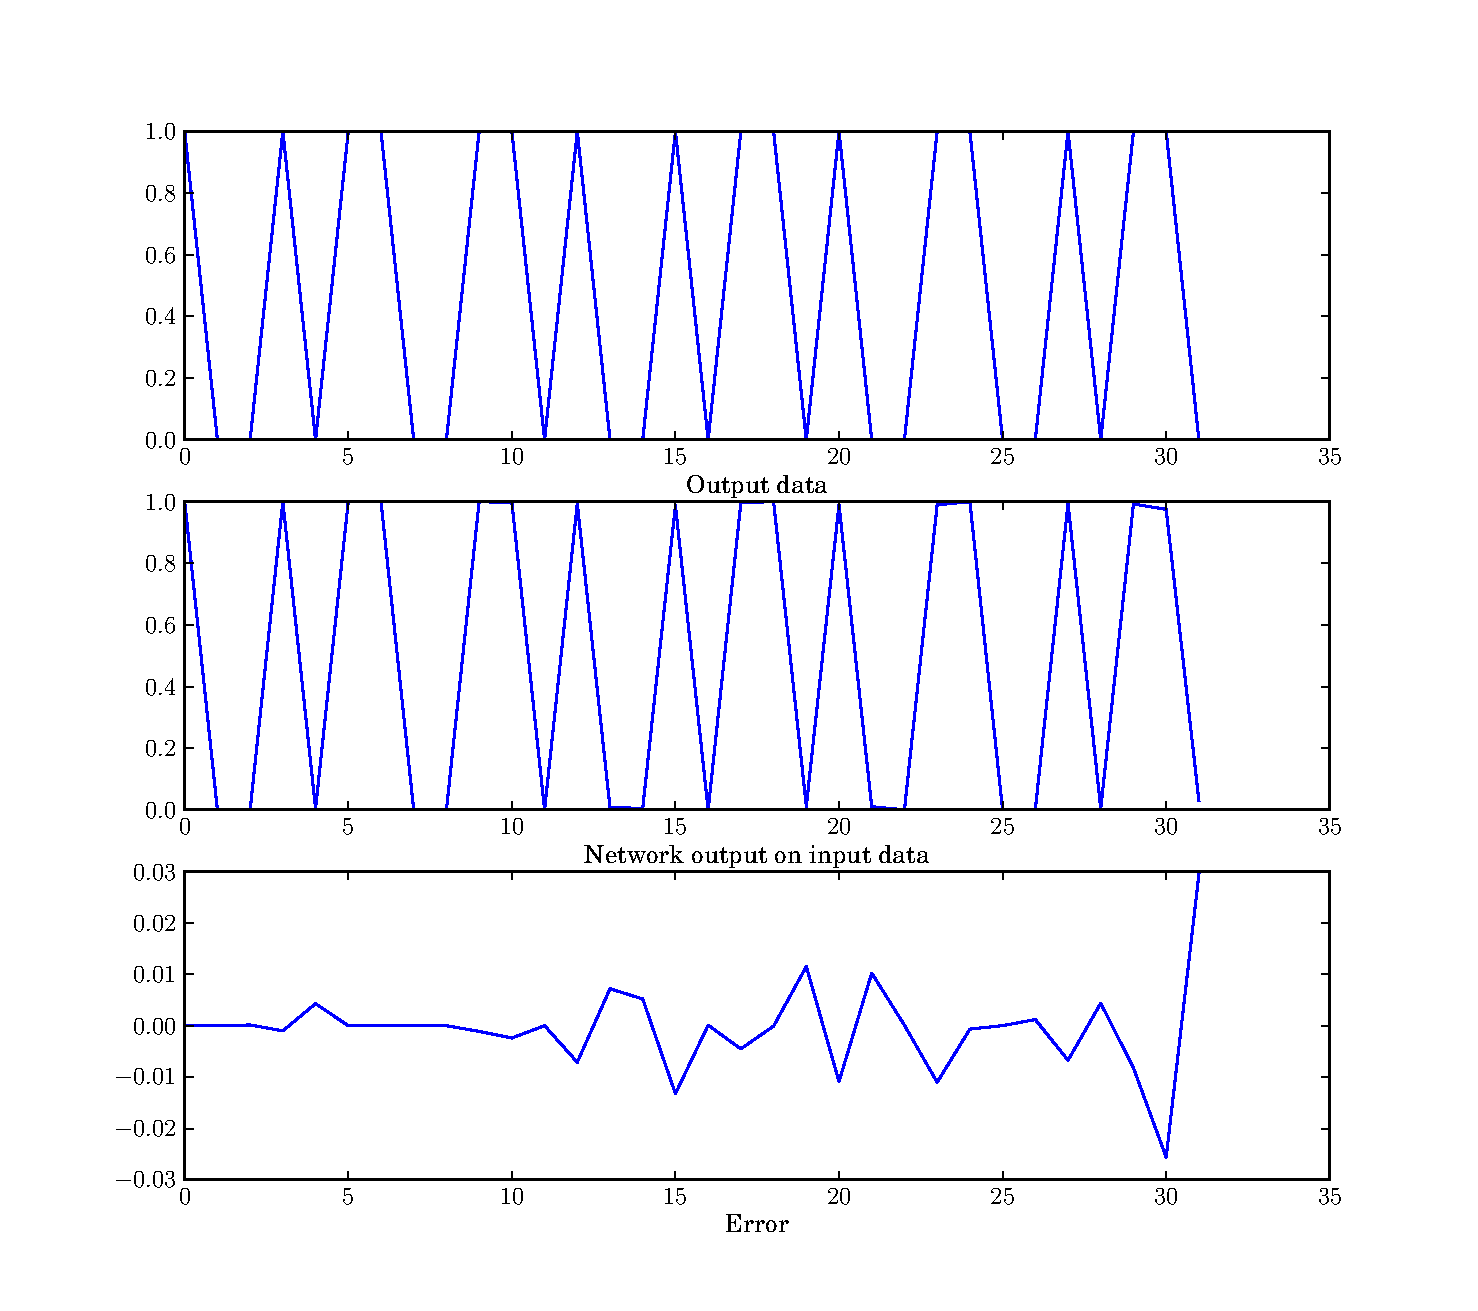
\includegraphics[scale=0.7]{src/parity.pdf}\caption{\label{fig:parity_result}Wyniki po uczeniu plików \texttt{parity}}
\end{figure}

\clearpage
\subsection{Plik \texttt{sincos}}

Dane okazały najmniejszy błąd za pomocą następujących funkcji aktywacji:
\begin{itemize}
\item Funkcja ukryta: sigmoidalna
\item Funkcja wyjściowa: tangencjalna
\item Ilość neuronów ukrytej warstwy: 40
\item Iteracje: 1000
\item Błąd: Poniżej 0.0004
\end{itemize}

\begin{table}[h]
\centering
\begin{tabular}[t]{c|c|l|l|l}
Funkcja ukryta & Funkcja wyjściowa & Ilość ukryta & Iteracje & Błąd \\
\hline
sigmoid & sigmoid & 5 & 1000 & 0.5 \\
sigmoid & sigmoid & 15 & 1000 & 0.5 \\
sigmoid & sigmoid & 40 & 1000 & 0.47 \\
sigmoid & tangential & 5 & 1000 & 0.0017 \\
sigmoid & tangential & 15 & 1000 & 0.0005 \\
sigmoid & tangential & 40 & 1000 & 0.0004 \\
sigmoid & linear & 5 & 1000 & 0.35 \\
sigmoid & linear & 15 & 1000 & 0.35 \\
sigmoid & linear & 40 & 1000 & 0.35 \\
linear & sigmoid & 5 & 1000 & 0.5 \\
linear & sigmoid & 15 & 1000 & 0.5 \\
linear & sigmoid & 40 & 1000 & 0.5 \\
linear & tangential & 5 & 1000 & 0.08 \\
linear & tangential & 15 & 1000 & 0.08 \\
linear & tangential & 40 & 1000 & 0.08 \\
linear & linear & 5 & 1000 & 0.35 \\
linear & linear & 15 & 1000 & 0.35 \\
linear & linear & 40 & 1000 & 0.35 \\
tangential & sigmoid & 5 & 1000 & 0.5 \\
tangential & sigmoid & 15 & 1000 & 0.5 \\
tangential & sigmoid & 40 & 1000 & 0.5 \\
tangential & tangential & 5 & 1000 & 0.0016 \\
tangential & tangential & 15 & 1000 & 0.0009 \\
tangential & tangential & 40 & 1000 & 0.0009 \\
tangential & linear & 5 & 1000 & 0.07 \\
tangential & linear & 15 & 1000 & 0.002 \\
tangential & linear & 40 & 1000 & 0.0006 \\
\end{tabular}
\caption{\label{tab:xor}Tablica prawdy bramki XOR}
\end{table}

\clearpage
\begin{figure}[!h]
\centering
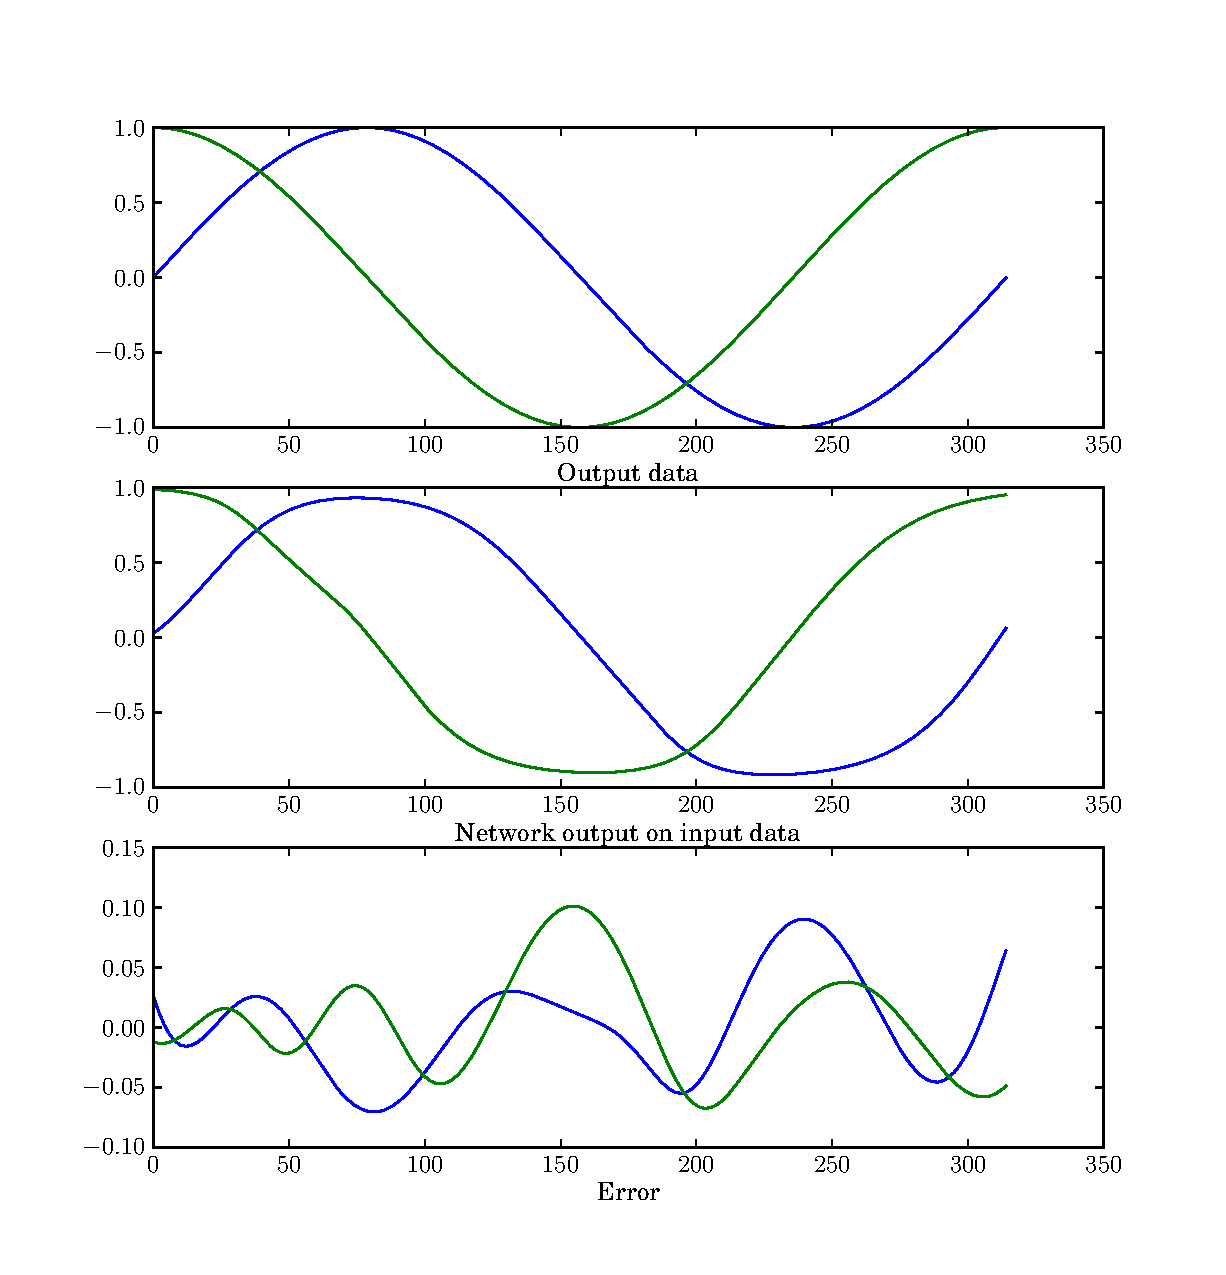
\includegraphics[scale=0.7]{src/sincos.pdf}\caption{\label{fig:xor_result}Wyniki po uczeniu}
\end{figure}

\clearpage
\subsection{Plik \texttt{glass.txt}}

Dane okazały najmniejszy błąd za pomocą następujących funkcji aktywacji:
\begin{itemize}
\item Funkcja ukryta: sigmoidalna
\item Funkcja wyjściowa: sigmoidalna
\item Ilość neuronów ukrytej warstwy: 40
\item Iteracje: 10000
\item Błąd: Poniżej 0.0004
\end{itemize}

Dla tego zestawu danych trzeba było dopisać nowa funkcje wczytania danych ponieważ wyjście i wejście znajdują się w tym samym pliku. Okazało się ze trzeba tez było drastycznie powiększyć maksymalna ilość iteracji aby osiągnąć sensownie niskie błędy sieci.

\begin{table}[h]
\centering
\begin{tabular}[t]{c|c|l|l|l}
Funkcja ukryta & Funkcja wyjściowa & Ilość ukryta & Iteracje & Błąd \\
\hline
sigmoid & sigmoid & 5 & 10000 & 0.05 \\
sigmoid & sigmoid & 15 & 10000 & 0.009 \\
sigmoid & sigmoid & 40 & 9229 & \\
sigmoid & tangential & 5 & 10000 & 0.013 \\
sigmoid & tangential & 15 & 10000 & 0.007 \\
sigmoid & tangential & 40 & 10000 & 0.004 \\
sigmoid & linear & 5 & 10000 & 0.06 \\
sigmoid & linear & 15 & 10000 & 0.03 \\
sigmoid & linear & 40 & 10000 & 0.017 \\
linear & sigmoid & 5 & 10000 & 0.069 \\
linear & sigmoid & 15 & 10000 & 0.069 \\
linear & sigmoid & 40 & 10000 & 0.069 \\
linear & tangential & 5 & 10000 & 0.02 \\
linear & tangential & 15 & 10000 & 0.02 \\
linear & tangential & 40 & 10000 & 0.02 \\
linear & linear & 5 & 10000 & 0.09 \\
linear & linear & 15 & 10000 & 0.08 \\
linear & linear & 40 & 10000 & 0.08 \\
tangential & sigmoid & 5 & 10000 & 0.04 \\
tangential & sigmoid & 15 & 10000 & 0.01 \\
tangential & sigmoid & 40 & 10000 & 0.007 \\
tangential & tangential & 5 & 10000 & 0.014 \\
tangential & tangential & 15 & 10000 & 0.01 \\
tangential & tangential & 40 & 10000 & 0.007 \\
tangential & linear & 5 & 10000 & 0.07 \\
tangential & linear & 15 & 10000 & 0.037 \\
tangential & linear & 40 & 10000 & 0.025 \\
\end{tabular}
\caption{\label{tab:xor}Tablica prawdy bramki XOR}
\end{table}

\clearpage
\begin{figure}[!h]
\centering
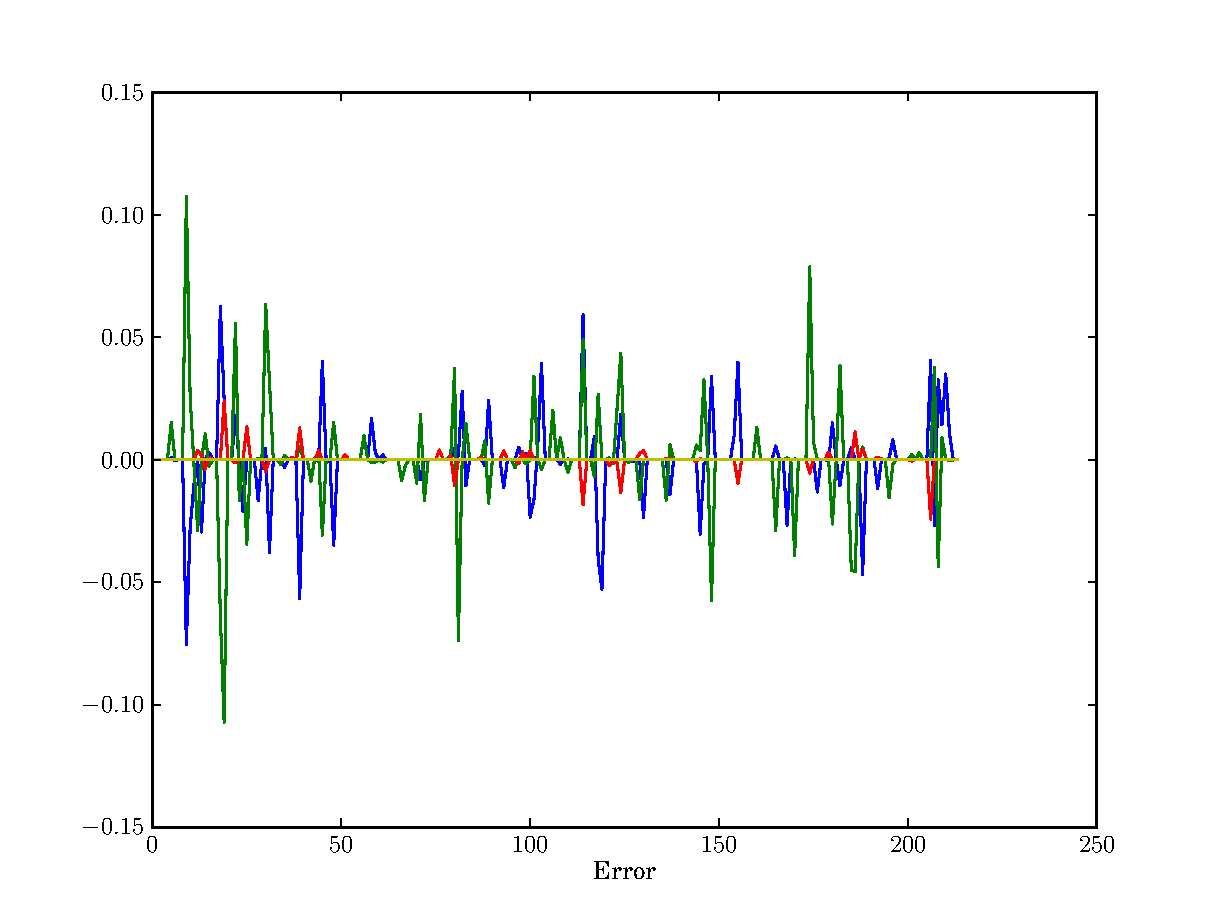
\includegraphics[scale=0.7]{src/glass.pdf}\caption{\label{fig:xor_result}Wyniki po uczeniu}
\end{figure}

\clearpage
\begin{center}
\lstset{captionpos=b,caption=Kod uczenia plików,label=lst:learn.py}
\lstinputlisting{src/learn.py}
\end{center}

\section{Podsumowanie}
Instalacja, nauczenie się funkcji dostępnych przez FANN, numpy i matplotlib pod Python zajęło dużo czasu ale zdaniem autora było warto. Nawet udało się w ramach tego sprawozdania znaleźć błąd biblioteki FANN, który występuje tylko przy wykorzystaniu języka Python. Autor biblioteki FANN został skontaktowany.

Pozostają jednak pytania dlaczego FANN stosunkowo źle się uczył w ramach sprawozdania zadanych danych.

\end{document}
